%==========================================================
% CHAPTER: Logaritmai ir eksponentinės funkcijos
%==========================================================
\chapter{Logaritmai ir eksponentinės funkcijos}

\section{Laipsnis ir šaknis}

Šiame skyriuje apibendrinsime laipsnio ir šaknies sąvokas, jų savybes bei
tarpusavio ryšius. Gebėjimas laisvai tvarkyti laipsnius ir šaknis yra vienas
iš svarbiausių VBE II dalies įgūdžių.

% ----------------------------------------------------------------
\subsection{Laipsnio savybės}
% ----------------------------------------------------------------

\begin{definition}[Laipsnis su natūraliuoju rodikliu]
Tegu $a \in \mathbb{R}$ ir $n \in \mathbb{N}$, $n \geq 1$. Skaičiaus $a$
\textbf{$n$-tasis laipsnis} apibrėžiamas kaip
\[
    a^n = \underbrace{a \cdot a \cdot \ldots \cdot a}_{n \text{ dauginamųjų}}.
\]
Skaičius $a$ vadinamas \textbf{laipsnio pagrindu}, skaičius $n$ –
\textbf{laipsnio rodikliu}.
\end{definition}

\begin{definition}[Nulinis ir neigiamas rodiklis]
Tegu $a \neq 0$. Apibrėžiame:
\[
    a^0 = 1, \qquad a^{-n} = \frac{1}{a^n}, \quad n \in \mathbb{N}.
\]
\end{definition}

\begin{remark}
Reiškinys $0^0$ matematikoje yra neapibrėžtas, o $0^{-n}$ neegzistuoja, nes
dalintume iš nulio.
\end{remark}

\subsubsection*{Pagrindinės laipsnių savybės}

Toliau pateikiamos savybės galioja visiems realiesiems skaičiams $a, b \neq 0$
ir sveikiesiems rodikliams $m, n \in \mathbb{Z}$ (jei nenurodyta kitaip).

\begin{tcolorbox}[title={Laipsnių savybės (santrauka)}, colback=blue!5!white,
                  colframe=blue!60!black]
\begin{enumerate}[label=\textbf{L\arabic*.}]
    \item $a^m \cdot a^n = a^{m+n}$
    \item $\dfrac{a^m}{a^n} = a^{m-n}$
    \item $(a^m)^n = a^{m \cdot n}$
    \item $(a \cdot b)^n = a^n \cdot b^n$
    \item $\left(\dfrac{a}{b}\right)^n = \dfrac{a^n}{b^n}$
\end{enumerate}
\end{tcolorbox}

\paragraph{L1. Sandaugos savybė (vienodų pagrindų laipsnių daugyba).}
\[
    a^m \cdot a^n = a^{m+n}.
\]
\textit{Įrodymas (natūraliesiems rodikliams).}
\[
    a^m \cdot a^n
    = \underbrace{a \cdot \ldots \cdot a}_{m} \cdot
      \underbrace{a \cdot \ldots \cdot a}_{n}
    = \underbrace{a \cdot \ldots \cdot a}_{m+n}
    = a^{m+n}. \qed
\]

\begin{example}
\[
    2^3 \cdot 2^5 = 2^{3+5} = 2^8 = 256.
\]
\[
    x^{-2} \cdot x^7 = x^{-2+7} = x^5.
\]
\end{example}

\paragraph{L2. Dalybos savybė (vienodų pagrindų laipsnių dalyba).}
\[
    \frac{a^m}{a^n} = a^{m-n}, \quad a \neq 0.
\]

\begin{example}
\[
    \frac{5^7}{5^3} = 5^{7-3} = 5^4 = 625.
\]
\[
    \frac{a^2}{a^5} = a^{2-5} = a^{-3} = \frac{1}{a^3}.
\]
\end{example}

\paragraph{L3. Laipsnio kėlimo laipsniu savybė.}
\[
    (a^m)^n = a^{m \cdot n}.
\]

\begin{example}
\[
    (3^2)^4 = 3^{8} = 6561.
\]
\[
    \left(x^{-3}\right)^2 = x^{-6} = \frac{1}{x^6}.
\]
\end{example}

\paragraph{L4. Sandaugos kėlimo laipsniu savybė.}
\[
    (a \cdot b)^n = a^n \cdot b^n.
\]

\begin{example}
\[
    (2 \cdot 3)^4 = 2^4 \cdot 3^4 = 16 \cdot 81 = 1296.
\]
\[
    (-2x^3)^3 = (-2)^3 \cdot (x^3)^3 = -8x^9.
\]
\end{example}

\paragraph{L5. Dalmenio kėlimo laipsniu savybė.}
\[
    \left(\frac{a}{b}\right)^n = \frac{a^n}{b^n}, \quad b \neq 0.
\]

\begin{example}
\[
    \left(\frac{3}{4}\right)^3 = \frac{27}{64}.
\]
\[
    \left(\frac{x^2}{y}\right)^4 = \frac{x^8}{y^4}.
\]
\end{example}

% ----------------------------------------------------------------
\subsubsection*{Laipsnis su racionaliuoju rodikliu}
% ----------------------------------------------------------------

\begin{definition}[Racionalusis rodiklis]
Tegu $a > 0$, $m \in \mathbb{Z}$, $n \in \mathbb{N}$, $n \geq 1$.
Apibrėžiame:
\[
    a^{\frac{m}{n}} = \sqrt[n]{a^m}.
\]
Ypatingas atvejis: $a^{\frac{1}{n}} = \sqrt[n]{a}$.
\end{definition}

\begin{remark}
Kai $a < 0$ ir $n$ yra lyginis skaičius, $a^{\frac{1}{n}}$ nėra apibrėžtas
realiuosiuose skaičiuose.
\end{remark}

Visos penkios laipsnių savybės (L1–L5) išlieka galioti ir racionaliesiems
rodikliams $m, n \in \mathbb{Q}$, kai pagrindas $a > 0$.

\begin{example}
Suprastinkite reiškinį $\dfrac{a^{\frac{3}{2}} \cdot a^{\frac{1}{2}}}{a^2}$.

\medskip
\textbf{Sprendimas:}
\[
    \frac{a^{\frac{3}{2}} \cdot a^{\frac{1}{2}}}{a^2}
    = \frac{a^{\frac{3}{2}+\frac{1}{2}}}{a^2}
    = \frac{a^{2}}{a^2}
    = a^{2-2} = a^0 = 1.
\]
\end{example}

\begin{example}
Apskaičiuokite $8^{\frac{2}{3}}$.

\medskip
\textbf{Sprendimas:}
\[
    8^{\frac{2}{3}} = \sqrt[3]{8^2} = \sqrt[3]{64} = 4.
\]
Arba:
\[
    8^{\frac{2}{3}} = \left(8^{\frac{1}{3}}\right)^2 = (\sqrt[3]{8})^2 = 2^2 = 4.
\]
\end{example}

% ----------------------------------------------------------------
\subsubsection*{Dažnos klaidos}
% ----------------------------------------------------------------

\begin{tcolorbox}[title={Dėmesio! Dažnos klaidos}, colback=red!5!white,
                  colframe=red!60!black]
\begin{itemize}
    \item $a^m \cdot b^m \neq (ab)^{2m}$ — dauginant skirtingų pagrindų
          laipsnius \textbf{negalima} sudėti rodiklių:
          $2^3 \cdot 3^3 = (2 \cdot 3)^3 = 6^3$, bet ne $6^6$.
    \item $a^m + a^n \neq a^{m+n}$ — laipsnių suma \textbf{nėra}
          laipsnis su sumos rodikliu:
          $2^3 + 2^2 = 8 + 4 = 12 \neq 2^5 = 32$.
    \item $(-a)^{2n} = a^{2n} \geq 0$ — lyginio laipsnio rezultatas
          visada \textbf{neneigiamas}.
    \item $(-a)^{2n+1} = -a^{2n+1}$ — nelyginio laipsnio rezultato
          ženklas sutampa su pagrindo ženklu.
\end{itemize}
\end{tcolorbox}

\begin{exercise}
Suprastinkite reiškinius:
\begin{enumerate}[label=\alph*)]
    \item $\dfrac{x^5 \cdot x^{-2}}{x^3}$
    \item $(2a^2b^{-1})^3 \cdot \dfrac{b^4}{4a^3}$
    \item $\left(\dfrac{27}{8}\right)^{-\frac{2}{3}}$
    \item $16^{0{,}75}$
\end{enumerate}
\end{exercise}

\begin{tcolorbox}[title={Atsakymai}, colback=green!5!white,
                  colframe=green!60!black]
a)~$1$;\quad b)~$2a^3b^3$;\quad
c)~$\left(\dfrac{8}{27}\right)^{\frac{2}{3}}
   = \dfrac{4}{9}$;\quad
d)~$16^{\frac{3}{4}} = (\sqrt[4]{16})^3 = 2^3 = 8$.
\end{tcolorbox}

% ================================================================
\subsection{Šaknies savybės}
% ================================================================

\begin{definition}[$n$-tojo laipsnio šaknis]
Tegu $n \in \mathbb{N}$, $n \geq 2$.
\begin{itemize}
    \item Jei $n$ yra \textbf{nelyginis}: $\sqrt[n]{a} = b \iff b^n = a$,
          $a, b \in \mathbb{R}$.
    \item Jei $n$ yra \textbf{lyginis}: $\sqrt[n]{a} = b \iff b^n = a$,
          $a \geq 0$, $b \geq 0$.
\end{itemize}
Ypatingas atvejis: $\sqrt{a} = \sqrt[2]{a}$ (kvadratinė šaknis).
\end{definition}

\begin{remark}
Iš neigiamo skaičiaus lyginės eilės šaknies traukti realiuosiuose skaičiuose
\textbf{negalima}: $\sqrt{-4}$ neegzistuoja $\mathbb{R}$ aibėje.
\end{remark}

\subsubsection*{Pagrindinės šaknų savybės}

\begin{tcolorbox}[title={Šaknų savybės (santrauka)}, colback=blue!5!white,
                  colframe=blue!60!black]
Tegu $a, b \geq 0$ (lyginei šakniai) arba $a, b \in \mathbb{R}$
(nelyginei šakniai), $n, m \in \mathbb{N}$, $n \geq 2$.
\begin{enumerate}[label=\textbf{Š\arabic*.}]
    \item $\sqrt[n]{a \cdot b} = \sqrt[n]{a} \cdot \sqrt[n]{b}$
    \item $\sqrt[n]{\dfrac{a}{b}} = \dfrac{\sqrt[n]{a}}{\sqrt[n]{b}},
          \quad b \neq 0$
    \item $\sqrt[n]{a^m} = \left(\sqrt[n]{a}\right)^m = a^{\frac{m}{n}}$
    \item $\sqrt[m]{\sqrt[n]{a}} = \sqrt[mn]{a}$
    \item $\sqrt[n]{a^n} = |a|$ (lyginiams $n$); \quad
          $\sqrt[n]{a^n} = a$ (nelyginiams $n$)
    \item $(\sqrt[n]{a})^n = a$, \quad $a \geq 0$
\end{enumerate}
\end{tcolorbox}

\paragraph{Š1. Sandaugos šaknis.}
\[
    \sqrt[n]{a \cdot b} = \sqrt[n]{a} \cdot \sqrt[n]{b}.
\]
\textit{Įrodymas.} Pažymėkime $\sqrt[n]{a} = p$ ir $\sqrt[n]{b} = q$.
Tada $p^n = a$, $q^n = b$, todėl:
\[
    \left(p \cdot q\right)^n = p^n \cdot q^n = a \cdot b
    \implies \sqrt[n]{ab} = pq = \sqrt[n]{a} \cdot \sqrt[n]{b}. \qed
\]

\begin{example}
\[
    \sqrt{12} = \sqrt{4 \cdot 3} = \sqrt{4} \cdot \sqrt{3} = 2\sqrt{3}.
\]
\[
    \sqrt[3]{54} = \sqrt[3]{27 \cdot 2} = 3\sqrt[3]{2}.
\]
\end{example}

\paragraph{Š2. Dalmenio šaknis.}
\[
    \sqrt[n]{\frac{a}{b}} = \frac{\sqrt[n]{a}}{\sqrt[n]{b}}, \quad b > 0.
\]

\begin{example}
\[
    \sqrt{\frac{25}{49}} = \frac{\sqrt{25}}{\sqrt{49}} = \frac{5}{7}.
\]
\[
    \sqrt[3]{\frac{x^6}{8}} = \frac{\sqrt[3]{x^6}}{\sqrt[3]{8}}
    = \frac{x^2}{2}.
\]
\end{example}

\paragraph{Š3. Šaknies ir laipsnio ryšys.}
\[
    \sqrt[n]{a^m} = a^{\frac{m}{n}}, \quad a > 0.
\]

\begin{example}
\[
    \sqrt[4]{a^6} = a^{\frac{6}{4}} = a^{\frac{3}{2}}
    = a \cdot \sqrt{a}, \quad a > 0.
\]
\[
    \sqrt[3]{x^{-2}} = x^{-\frac{2}{3}} = \frac{1}{\sqrt[3]{x^2}},
    \quad x > 0.
\]
\end{example}

\paragraph{Š4. Šaknies iš šaknies traukimas.}
\[
    \sqrt[m]{\sqrt[n]{a}} = \sqrt[mn]{a}.
\]

\begin{example}
\[
    \sqrt{\sqrt[3]{64}} = \sqrt[6]{64} = 64^{\frac{1}{6}}
    = (2^6)^{\frac{1}{6}} = 2.
\]
\end{example}

\paragraph{Š5. Laipsnio ir šaknies sutraukimas.}
\[
    \sqrt[n]{a^n} =
    \begin{cases}
        |a|, & \text{jei } n \text{ lyginis}, \\
        a,   & \text{jei } n \text{ nelyginis}.
    \end{cases}
\]

\begin{example}
\[
    \sqrt{(-5)^2} = \sqrt{25} = 5 = |-5|.
\]
\[
    \sqrt[3]{(-2)^3} = \sqrt[3]{-8} = -2.
\]
\end{example}

\begin{remark}
Svarbu nepainioti: $\sqrt{a^2} = |a|$, \textbf{ne} $a$!
Pvz.: $\sqrt{(-3)^2} = |-3| = 3 \neq -3$.
\end{remark}

% ----------------------------------------------------------------
\subsubsection*{Šaknies iškėlimas iš po šaknies ženklo ir
                įnešimas po juo}
% ----------------------------------------------------------------

Dažnai reikia \textbf{supaprastinti} reiškinius, susijusius su šaknimis.

\begin{example}[Iškėlimas iš po šaknies ženklo]
Suprastinkite $\sqrt{72}$.
\[
    \sqrt{72} = \sqrt{36 \cdot 2} = 6\sqrt{2}.
\]
Arba:
\[
    \sqrt{72} = \sqrt{4 \cdot 18} = 2\sqrt{18} = 2\sqrt{9 \cdot 2}
    = 2 \cdot 3\sqrt{2} = 6\sqrt{2}.
\]
\end{example}

\begin{example}[Įnešimas po šaknies ženklu]
Užrašykite $3\sqrt{5}$ kaip vieną šaknį.
\[
    3\sqrt{5} = \sqrt{9} \cdot \sqrt{5} = \sqrt{45}.
\]
\end{example}

% ----------------------------------------------------------------
\subsubsection*{Šaknies panaikinimas vardiklyje (racionalizavimas)}
% ----------------------------------------------------------------

VBE užduotyse dažnai reikalaujama \textbf{pašalinti šaknį iš trupmenos
vardiklio}.

\begin{tcolorbox}[title={Racionalizavimo formulės},
                  colback=yellow!10!white, colframe=orange!80!black]
\begin{align*}
    \frac{c}{\sqrt{a}} &= \frac{c\sqrt{a}}{a}, \\[6pt]
    \frac{c}{\sqrt{a} \pm \sqrt{b}}
    &= \frac{c\left(\sqrt{a} \mp \sqrt{b}\right)}{a - b}.
\end{align*}
\end{tcolorbox}

\begin{example}
\[
    \frac{6}{\sqrt{3}} = \frac{6\sqrt{3}}{3} = 2\sqrt{3}.
\]
\end{example}

\begin{example}
\[
    \frac{1}{\sqrt{5}+\sqrt{2}}
    = \frac{\sqrt{5}-\sqrt{2}}{(\sqrt{5})^2-(\sqrt{2})^2}
    = \frac{\sqrt{5}-\sqrt{2}}{5-2}
    = \frac{\sqrt{5}-\sqrt{2}}{3}.
\]
\end{example}

% ----------------------------------------------------------------
\subsubsection*{Sudėtingesni pavyzdžiai}
% ----------------------------------------------------------------

\begin{example}
Suprastinkite:
\[
    \frac{\sqrt[3]{a^4} \cdot \sqrt{a}}{\sqrt[6]{a^5}},
    \quad a > 0.
\]
\textbf{Sprendimas.} Verskime viską laipsniais su racionaliaisiais rodikliais:
\[
    \frac{a^{\frac{4}{3}} \cdot a^{\frac{1}{2}}}{a^{\frac{5}{6}}}
    = a^{\frac{4}{3} + \frac{1}{2} - \frac{5}{6}}
    = a^{\frac{8}{6} + \frac{3}{6} - \frac{5}{6}}
    = a^{\frac{6}{6}}
    = a^1 = a.
\]
\end{example}

\begin{example}
Apskaičiuokite:
\[
    \left(\frac{1}{4}\right)^{-\frac{3}{2}}.
\]
\textbf{Sprendimas:}
\[
    \left(\frac{1}{4}\right)^{-\frac{3}{2}}
    = \left(\frac{4}{1}\right)^{\frac{3}{2}}
    = 4^{\frac{3}{2}}
    = \left(\sqrt{4}\right)^3
    = 2^3 = 8.
\]
\end{example}

% ----------------------------------------------------------------
\subsubsection*{Uždaviniai savarankiškam darbui}
% ----------------------------------------------------------------

\begin{exercise}
Suprastinkite:
\begin{enumerate}[label=\alph*)]
    \item $\sqrt{50} - \sqrt{18} + \sqrt{8}$
    \item $\dfrac{1}{\sqrt{7}-\sqrt{3}}$
    \item $\sqrt[4]{16x^8y^{12}}$, \quad $x, y > 0$
    \item $\left(\sqrt{a} - \dfrac{1}{\sqrt{a}}\right)^2$, \quad $a > 0$
    \item $\dfrac{\sqrt[3]{a^2} \cdot \sqrt[6]{a}}{\sqrt{a}}$,
          \quad $a > 0$
\end{enumerate}
\end{exercise}

\begin{tcolorbox}[title={Atsakymai}, colback=green!5!white,
                  colframe=green!60!black]
a)~$4\sqrt{2}$;\quad
b)~$\dfrac{\sqrt{7}+\sqrt{3}}{4}$;\quad
c)~$2x^2y^3$;\quad
d)~$a - 2 + \dfrac{1}{a}$;\quad
e)~$a^{\frac{2}{3}+\frac{1}{6}-\frac{1}{2}} = a^{\frac{1}{3}} = \sqrt[3]{a}$.
\end{tcolorbox}


\section{Eksponentinė funkcija}

\subsection{Apibrėžimas ir savybės}

\begin{definition}
Funkcija $f(x) = a^x$, kur $a > 0$ ir $a \neq 1$, $x \in \mathbb{R}$, vadinama
\textbf{eksponentine funkcija} su pagrindu $a$.
\end{definition}

\begin{remark}
Sąlyga $a \neq 1$ būtina, nes $f(x) = 1^x = 1$ yra pastovioji funkcija, o ne
eksponentinė. Sąlyga $a > 0$ užtikrina, kad $a^x$ būtų apibrėžta visiems
realiesiems $x$.
\end{remark}

Svarbus eksponentinės funkcijos atvejis yra \textbf{natūralioji eksponentė}:
\[
f(x) = e^x = \exp(x),
\]
kur $e \approx 2{,}71828\ldots$ yra Eulerio skaičius --- matematinė konstanta,
kuri pasitaiko daugelyje gamtos ir ekonomikos modelių.

\subsubsection*{Pagrindinės savybės}

Tarkime, kad $f(x) = a^x$.

\begin{enumerate}[label=\arabic*.]
    \item \textbf{Apibrėžimo sritis:} $D(f) = \mathbb{R} = (-\infty; +\infty)$.
    \item \textbf{Reikšmių sritis:} $E(f) = (0; +\infty)$ --- funkcija visada
          teigiama.
    \item \textbf{Monotoniškumas:}
        \begin{itemize}
            \item Jei $a > 1$, tai $f(x) = a^x$ \textit{didėja} visoje
                  apibrėžimo srityje.
            \item Jei $0 < a < 1$, tai $f(x) = a^x$ \textit{mažėja} visoje
                  apibrėžimo srityje.
        \end{itemize}
    \item \textbf{Fiksuotas taškas:} $f(0) = a^0 = 1$ visiems leistiniems
          pagrindams $a$, t.~y. grafiko ir $y$\nobreakdash-ašies susikirtimo
          taškas visada yra $(0,\,1)$.
    \item \textbf{Horizontali asimptota:} $y = 0$ (x ašis).
        \begin{itemize}
            \item Jei $a > 1$: $\lim_{x \to -\infty} a^x = 0$ ir
                  $\lim_{x \to +\infty} a^x = +\infty$.
            \item Jei $0 < a < 1$: $\lim_{x \to +\infty} a^x = 0$ ir
                  $\lim_{x \to -\infty} a^x = +\infty$.
        \end{itemize}
    \item \textbf{Funkcija nei lyginė, nei nelyginė.}
    \item \textbf{Nėra periodinė.}
    \item \textbf{Funkcija tolydi} visoje $\mathbb{R}$.
\end{enumerate}

\subsubsection*{Laipsnių savybės (taikomos eksponentinei funkcijai)}

Kadangi $f(x) = a^x$ remiasi kėlimu laipsniu, galioja šios taisyklės:

\begin{align}
    a^{x+y} &= a^x \cdot a^y, \\
    a^{x-y} &= \frac{a^x}{a^y}, \\
    \left(a^x\right)^y &= a^{xy}, \\
    (ab)^x &= a^x \cdot b^x.
\end{align}

\begin{example}
Apskaičiuokite $2^3 \cdot 2^5$.
\[
    2^3 \cdot 2^5 = 2^{3+5} = 2^8 = 256.
\]
\end{example}

\begin{example}
Suprastinkite reiškinį $\dfrac{3^{2x}}{3^x}$.
\[
    \frac{3^{2x}}{3^x} = 3^{2x - x} = 3^x.
\]
\end{example}

\begin{tcolorbox}[title=Pagrindų palyginimas]
\centering
\begin{tabular}{|l|c|c|}
\hline
\textbf{Savybė} & $a > 1$ & $0 < a < 1$ \\
\hline
Monotoniškumas & didėjanti & mažėjanti \\
$x \to +\infty$ & $f(x) \to +\infty$ & $f(x) \to 0$ \\
$x \to -\infty$ & $f(x) \to 0$ & $f(x) \to +\infty$ \\
Horizontali asimptota & $y = 0$ iš kairės & $y = 0$ iš dešinės \\
\hline
\end{tabular}
\end{tcolorbox}

\begin{exercise}
Nustatykite, ar funkcija $f(x) = \left(\tfrac{1}{3}\right)^x$ didėjanti ar
mažėjanti. Pagrįskite atsakymą.
\end{exercise}

\begin{exercise}
Apskaičiuokite: $\dfrac{5^{3x+2}}{5^{3x-1}}$.
\end{exercise}

% ----------------------------------------------------------------
\subsection{Grafikas ir transformacijos}

\subsubsection*{Pagrindiniai grafikai}

Eksponentinės funkcijos $f(x) = a^x$ grafikas priklauso nuo pagrindo $a$:

\begin{center}
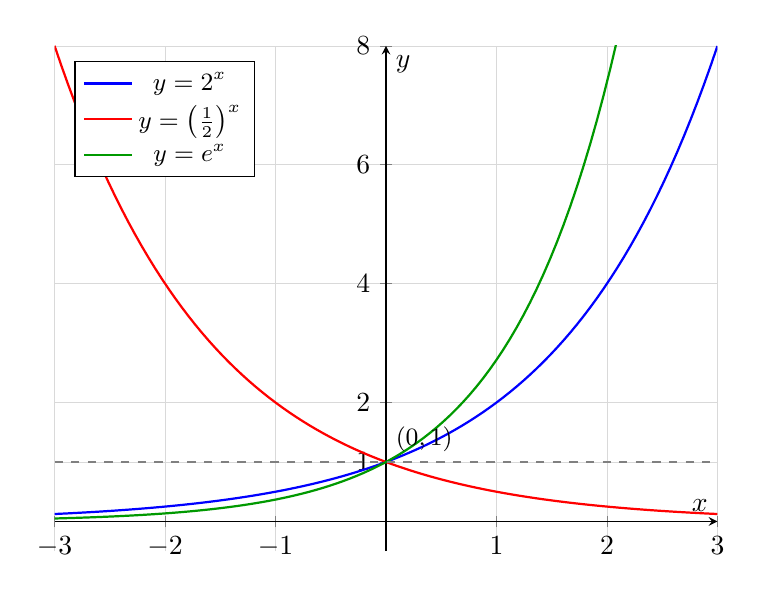
\begin{tikzpicture}
\begin{axis}[
    axis lines = center,
    xlabel = {$x$},
    ylabel = {$y$},
    xmin=-3, xmax=3,
    ymin=-0.5, ymax=8,
    xtick={-3,-2,-1,0,1,2,3},
    ytick={1,2,4,6,8},
    legend pos=north west,
    legend style={font=\small},
    grid=both,
    grid style={line width=0.2pt, draw=gray!30},
    width=10cm, height=8cm,
]
\addplot[thick, blue, domain=-3:3, samples=100] {2^x};
\addlegendentry{$y = 2^x$}

\addplot[thick, red, domain=-3:3, samples=100] {(0.5)^x};
\addlegendentry{$y = \left(\frac{1}{2}\right)^x$}

\addplot[thick, green!60!black, domain=-3:3, samples=100] {exp(x)};
\addlegendentry{$y = e^x$}

\addplot[dashed, gray, domain=-3:3] {1};
\node[above right] at (axis cs:0,1) {\small$(0,1)$};
\end{axis}
\end{tikzpicture}
\end{center}

\begin{remark}
Visi trys grafikai kerta $y$\nobreakdash-ašį taške $(0, 1)$. Funkcija
$y = \left(\tfrac{1}{2}\right)^x$ yra funkcijos $y = 2^x$ atspindys $y$\nobreakdash-ašies
atžvilgiu, nes $\left(\tfrac{1}{2}\right)^x = 2^{-x}$.
\end{remark}

\subsubsection*{Transformacijos}

Bendroji transformuotos eksponentinės funkcijos forma:
\[
    f(x) = c \cdot a^{k(x - h)} + d,
\]
kur $h$ --- horizontalusis poslinkis, $d$ --- vertikalusis poslinkis,
$c$ --- vertikalusis ištempimas (arba suspaudimas), $k$ --- horizontalusis
ištempimas (arba suspaudimas).

\paragraph{1. Vertikalusis poslinkis.}
\[
    g(x) = a^x + d
\]
Grafikas pastumamas \textit{aukštyn} $d$ vienetų, jei $d > 0$, arba
\textit{žemyn} $|d|$ vienetų, jei $d < 0$.
Horizontali asimptota tampa $y = d$.

\begin{example}
$g(x) = 2^x + 3$ --- funkcijos $y = 2^x$ grafikas pastumtas aukštyn 3 vienetais.
Horizontali asimptota: $y = 3$.
\end{example}

\paragraph{2. Horizontalusis poslinkis.}
\[
    g(x) = a^{x - h}
\]
Grafikas pastumamas \textit{į dešinę} $h$ vienetų, jei $h > 0$, arba
\textit{į kairę} $|h|$ vienetų, jei $h < 0$.

\begin{example}
$g(x) = 2^{x-2}$ --- funkcijos $y = 2^x$ grafikas pastumtas į dešinę 2 vienetais.
Taškas $(0, 1)$ perkeliamas į $(2, 1)$.
\end{example}

\paragraph{3. Atspindys.}
\begin{itemize}
    \item \textbf{Atspindys $x$\nobreakdash-ašies atžvilgiu:}
          $g(x) = -a^x$ --- grafikas apverčiamas žemyn.
    \item \textbf{Atspindys $y$\nobreakdash-ašies atžvilgiu:}
          $g(x) = a^{-x}$ --- grafikas atspindimas horizontaliai.
\end{itemize}

\begin{example}
$g(x) = -2^x$: visos reikšmės teigiamos paverčiamos neigiamomis.
Reikšmių sritis tampa $(-\infty;\, 0)$.
\end{example}

\paragraph{4. Vertikalusis ištempimas ir suspaudimas.}
\[
    g(x) = c \cdot a^x
\]
\begin{itemize}
    \item Jei $c > 1$: grafikas \textit{ištemptas vertikaliai} $c$ kartų.
    \item Jei $0 < c < 1$: grafikas \textit{suspaustas vertikaliai}.
    \item Taškas $(0, 1)$ perkeliamas į $(0, c)$.
\end{itemize}

\paragraph{5. Horizontalusis ištempimas ir suspaudimas.}
\[
    g(x) = a^{kx}
\]
\begin{itemize}
    \item Jei $|k| > 1$: grafikas \textit{suspaustas horizontaliai}.
    \item Jei $0 < |k| < 1$: grafikas \textit{ištemptas horizontaliai}.
\end{itemize}

\subsubsection*{Transformacijų santrauka}

\begin{tcolorbox}[title={Eksponentinės funkcijos $y = a^x$ transformacijos}]
\centering
\renewcommand{\arraystretch}{1.4}
\begin{tabular}{|l|l|l|}
\hline
\textbf{Transformacija} & \textbf{Formulė} & \textbf{Poveikis grafikui} \\
\hline
Vertikalusis poslinkis & $a^x + d$ & Aukštyn / žemyn $d$ vienetų \\
Horizontalusis poslinkis & $a^{x-h}$ & Dešinėn / kairėn $h$ vienetų \\
Atspindys per $x$-ašį & $-a^x$ & Apverčia žemyn \\
Atspindys per $y$-ašį & $a^{-x}$ & Atspindi horizontaliai \\
Vert. ištempimas & $c \cdot a^x,\ c > 1$ & Ištempimas $c$ kartų \\
Vert. suspaudimas & $c \cdot a^x,\ 0 < c < 1$ & Suspaudimas \\
Horiz. suspaudimas & $a^{kx},\ |k|>1$ & Suspaudimas \\
Horiz. ištempimas & $a^{kx},\ 0<|k|<1$ & Ištempimas \\
\hline
\end{tabular}
\end{tcolorbox}

\begin{exercise}
Nubraižykite funkcijų $y = 3^x$, $y = 3^x - 2$ ir $y = 3^{x+1}$ grafikus
vienoje koordinačių sistemoje. Nurodykite kiekvieno grafiko horizontalią
asimptotą ir tašką, kuriame grafikas kerta $y$-ašį.
\end{exercise}

\begin{exercise}
Funkcijos $f(x) = 2^x$ grafiko pagrindu nubrėžkite funkcijos
$g(x) = -2^{x-1} + 4$ grafiką. Nurodykite:
\begin{enumerate}[label=\alph*)]
    \item Horizontalios asimptotos lygtį.
    \item Reikšmių sritį.
    \item $y$-ašies susikirtimo tašką.
\end{enumerate}
\end{exercise}


\section{Logaritmas}

\subsection{Logaritmo apibrėžimas}

\begin{definition}
Tegu $a > 0$, $a \neq 1$ ir $b > 0$. \textbf{Skaičiaus $b$ logaritmu pagrindu $a$} vadinamas rodiklis, kuriuo reikia pakelti skaičių $a$, kad gautume $b$. Žymima $\log_a b$.
\[
\log_a b = c \iff a^c = b, \quad a > 0,\ a \neq 1,\ b > 0.
\]
\end{definition}

\begin{remark}
Logaritmo egzistavimo sąlygos:
\begin{itemize}
    \item Pagrindas $a$ turi būti teigiamas ir ne lygus vienetui: $a > 0$, $a \neq 1$.
    \item Argumentas $b$ turi būti teigiamas: $b > 0$.
    \item Neigiamų skaičių ir nulio logaritmas \textbf{neegzistuoja}.
\end{itemize}
\end{remark}

Logaritmas ir laipsnio kėlimas yra \textbf{atvirkštinės operacijos}. Galima taip interpretuoti:
\[
\log_a b = c \quad \Longleftrightarrow \quad a^c = b.
\]

\begin{example}
Apskaičiuokite šiuos logaritmus:
\begin{enumerate}[label=\alph*)]
    \item $\log_2 8 = ?$ \quad Nes $2^3 = 8$, tai $\log_2 8 = 3$.
    \item $\log_3 81 = ?$ \quad Nes $3^4 = 81$, tai $\log_3 81 = 4$.
    \item $\log_5 1 = ?$ \quad Nes $5^0 = 1$, tai $\log_5 1 = 0$.
    \item $\log_4 \frac{1}{16} = ?$ \quad Nes $4^{-2} = \frac{1}{16}$, tai $\log_4 \frac{1}{16} = -2$.
    \item $\log_9 3 = ?$ \quad Nes $9^{1/2} = 3$, tai $\log_9 3 = \frac{1}{2}$.
\end{enumerate}
\end{example}

\begin{tcolorbox}[title=Pagrindinė logaritmo tapatybė]
Iš apibrėžimo tiesiogiai išplaukia \textbf{pagrindinė logaritmo tapatybė}:
\[
a^{\log_a b} = b, \quad a > 0,\ a \neq 1,\ b > 0.
\]
Taip pat:
\[
\log_a a^n = n, \quad \log_a 1 = 0, \quad \log_a a = 1.
\]
\end{tcolorbox}

\begin{proof}[Įrodymas ($\log_a 1 = 0$)]
Pagal apibrėžimą, $\log_a 1 = c \iff a^c = 1$. Nes $a^0 = 1$ bet kuriam $a \neq 0$, tai $c = 0$. Vadinasi $\log_a 1 = 0$. $\square$
\end{proof}

\begin{exercise}
Nustatykite, ar šie logaritmai egzistuoja, ir jei taip – apskaičiuokite:
\begin{enumerate}[label=\arabic*.]
    \item $\log_3 (-9)$
    \item $\log_1 5$
    \item $\log_{1/2} 4$
    \item $\log_6 \sqrt{6}$
    \item $\log_{0{,}1} 10$
\end{enumerate}
\end{exercise}

% -------------------------------------------------------
\subsection{Logaritmo savybės}

Toliau pateikiamos pagrindinės logaritmų savybės. Jos galioja, kai $a > 0$, $a \neq 1$, $b > 0$, $c > 0$.

\begin{tcolorbox}[title=Pagrindinės logaritmų savybės]
\begin{enumerate}[label=\textbf{\arabic*.}]
    \item \textbf{Sandaugos logaritmas:}
    \[
    \log_a (b \cdot c) = \log_a b + \log_a c
    \]
    \item \textbf{Dalinės logaritmas:}
    \[
    \log_a \frac{b}{c} = \log_a b - \log_a c
    \]
    \item \textbf{Laipsnio logaritmas:}
    \[
    \log_a b^n = n \cdot \log_a b, \quad n \in \mathbb{R}
    \]
    \item \textbf{Pagrindo keitimo formulė:}
    \[
    \log_a b = \frac{\log_k b}{\log_k a}, \quad k > 0,\ k \neq 1
    \]
\end{enumerate}
\end{tcolorbox}

\subsubsection*{Savybių įrodymai}

\begin{proof}[Įrodymas (sandaugos savybė)]
Tegu $\log_a b = m$ ir $\log_a c = n$. Tada $a^m = b$ ir $a^n = c$.\\
Tuomet:
\[
b \cdot c = a^m \cdot a^n = a^{m+n}.
\]
Pagal logaritmo apibrėžimą: $\log_a(b \cdot c) = m + n = \log_a b + \log_a c$. $\square$
\end{proof}

\begin{proof}[Įrodymas (laipsnio savybė)]
Tegu $\log_a b = m$, tada $a^m = b$.\\
Tuomet:
\[
b^n = (a^m)^n = a^{mn}.
\]
Pagal logaritmo apibrėžimą: $\log_a b^n = mn = n \cdot \log_a b$. $\square$
\end{proof}

\begin{proof}[Įrodymas (pagrindo keitimo formulė)]
Tegu $\log_a b = t$, tada $a^t = b$.\\
Pritaikome logaritmą $\log_k$ abiem pusėms:
\[
\log_k(a^t) = \log_k b \implies t \cdot \log_k a = \log_k b \implies t = \frac{\log_k b}{\log_k a}.
\]
Vadinasi $\log_a b = \dfrac{\log_k b}{\log_k a}$. $\square$
\end{proof}

\begin{remark}
Iš pagrindo keitimo formulės išplaukia naudinga savybė:
\[
\log_a b \cdot \log_b a = 1 \implies \log_a b = \frac{1}{\log_b a}.
\]
\end{remark}

\begin{example}
Supaprastinkite reiškinį $\log_2 6 + \log_2 \frac{4}{3}$:
\[
\log_2 6 + \log_2 \frac{4}{3} = \log_2 \left(6 \cdot \frac{4}{3}\right) = \log_2 8 = \log_2 2^3 = 3.
\]
\end{example}

\begin{example}
Apskaičiuokite $\log_4 32$ naudodami pagrindo keitimą:
\[
\log_4 32 = \frac{\log_2 32}{\log_2 4} = \frac{5}{2}.
\]
\end{example}

\begin{example}
Supaprastinkite: $\log_3 \frac{\sqrt{27}}{9}$:
\[
\log_3 \frac{\sqrt{27}}{9} = \log_3 \sqrt{27} - \log_3 9 = \log_3 3^{3/2} - \log_3 3^2 = \frac{3}{2} - 2 = -\frac{1}{2}.
\]
\end{example}

\begin{exercise}
Supaprastinkite arba apskaičiuokite:
\begin{enumerate}[label=\arabic*.]
    \item $\log_5 50 + \log_5 2 - \log_5 4$
    \item $\log_2 3 \cdot \log_3 16$
    \item $3\log_6 2 + \log_6 27 - \log_6 \frac{3}{2}$
    \item $\log_8 4 + \log_8 16$
    \item $\dfrac{\log 125}{\log 5}$
\end{enumerate}
\end{exercise}

% -------------------------------------------------------
\subsection{Dešimtainis ir natūralusis logaritmas}

Praktikoje dažniausiai naudojami du specialūs logaritmai – dešimtainis ir natūralusis.

\begin{definition}
\textbf{Dešimtainis logaritmas} – tai logaritmas, kurio pagrindas yra $10$. Žymimas $\lg b$ arba $\log b$ (be pagrindo):
\[
\lg b = \log_{10} b.
\]
\end{definition}

\begin{definition}
\textbf{Natūralusis logaritmas} – tai logaritmas, kurio pagrindas yra Eulerio skaičius $e \approx 2{,}71828\ldots$ Žymimas $\ln b$:
\[
\ln b = \log_e b.
\]
\end{definition}

\begin{remark}
Eulerio skaičius $e$ yra iracionalusis skaičius. Jis apibrėžiamas kaip:
\[
e = \lim_{n \to \infty} \left(1 + \frac{1}{n}\right)^n \approx 2{,}71828\ldots
\]
Natūralusis logaritmas itin svarbus analizėje, nes $(\ln x)' = \dfrac{1}{x}$.
\end{remark}

\begin{tcolorbox}[title=Specialiosios reikšmės]
\begin{center}
\begin{tabular}{|c|c|c|}
\hline
\textbf{Reiškinys} & \textbf{Reikšmė} & \textbf{Pagrindimas} \\
\hline
$\lg 1$ & $0$ & $10^0 = 1$ \\
$\lg 10$ & $1$ & $10^1 = 10$ \\
$\lg 100$ & $2$ & $10^2 = 100$ \\
$\lg 0{,}1$ & $-1$ & $10^{-1} = 0{,}1$ \\
$\ln 1$ & $0$ & $e^0 = 1$ \\
$\ln e$ & $1$ & $e^1 = e$ \\
$\ln e^k$ & $k$ & $e^k = e^k$ \\
\hline
\end{tabular}
\end{center}
\end{tcolorbox}

\begin{example}
Apskaičiuokite $\lg 0{,}001$:
\[
\lg 0{,}001 = \lg 10^{-3} = -3.
\]
\end{example}

\begin{example}
Supaprastinkite $e^{3\ln 2}$:
\[
e^{3\ln 2} = e^{\ln 2^3} = e^{\ln 8} = 8.
\]
\end{example}

\begin{example}
Išreikškite $\log_3 7$ per dešimtainius logaritmus:
\[
\log_3 7 = \frac{\lg 7}{\lg 3} \approx \frac{0{,}8451}{0{,}4771} \approx 1{,}771.
\]
\end{example}

\begin{remark}
VBE egzamino metu leidžiama naudotis formulynu, kuriame pateikiamos visos pagrindinės logaritmų savybės. Tačiau svarbu mokėti jas taikyti be klaidų sprendžiant lygtis ir supaprastinant reiškinius.
\end{remark}

\begin{exercise}
Išspręskite ir supaprastinkite:
\begin{enumerate}[label=\arabic*.]
    \item Apskaičiuokite: $\lg 4 + \lg 25$.
    \item Apskaičiuokite: $\ln e^5 - \ln e^2$.
    \item Išreikškite $\log_7 3$ per natūraliuosius logaritmus.
    \item Supaprastinkite: $10^{2 + \lg 3}$.
    \item Raskite $x$, jei $\ln x = 3$.
\end{enumerate}
\end{exercise}


\section{Logaritminė funkcija}

\subsection{Apibrėžimas ir savybės}

\begin{definition}
Tegu $a > 0$ ir $a \neq 1$. \textbf{Logaritmine baze $a$} vadinama funkcija
\[
f(x) = \log_a x, \quad x > 0,
\]
kuri kiekvienam teigiamuoju skaičiui $x$ priskiria tokį laipsnį $y$, kad $a^y = x$.
\end{definition}

Kitaip tariant, $y = \log_a x \iff a^y = x$. Logaritminė funkcija yra atvirkštinė eksponentinei funkcijai $g(x) = a^x$ [web:3][web:9].

\begin{remark}
Dvi ypatingos logaritminės funkcijos:
\begin{itemize}
  \item \textbf{Dešimtainis logaritmas:} $f(x) = \log_{10} x = \lg x$ (bazė $a = 10$) [web:7].
  \item \textbf{Natūralusis logaritmas:} $f(x) = \log_e x = \ln x$, kur $e \approx 2{,}71828$ yra Eulerio skaičius [web:7][web:9].
\end{itemize}
\end{remark}

\subsubsection*{Apibrėžimo ir reikšmių sritis}

\begin{itemize}
  \item \textbf{Apibrėžimo sritis:} $D(f) = (0; +\infty)$, nes logaritmą galima skaičiuoti tik iš teigiamų skaičių [web:5][web:9].
  \item \textbf{Reikšmių sritis:} $E(f) = (-\infty; +\infty) = \mathbb{R}$ – logaritminė funkcija įgyja visas realiąsias reikšmes [web:5][web:7].
\end{itemize}

\subsubsection*{Logaritmų savybės (taisyklės)}

Tegu $a > 0$, $a \neq 1$, $M > 0$, $N > 0$, $p \in \mathbb{R}$. Tuomet galioja šios pagrindinės logaritmų savybės [web:5][web:9]:

\begin{tcolorbox}[title={Pagrindinės logaritmų savybės}]
\begin{enumerate}[label=\arabic*.]
  \item \textbf{Sandaugos taisyklė:}
  \[
    \log_a(M \cdot N) = \log_a M + \log_a N
  \]
  \item \textbf{Dalyba:}
  \[
    \log_a\!\left(\frac{M}{N}\right) = \log_a M - \log_a N
  \]
  \item \textbf{Laipsnio taisyklė:}
  \[
    \log_a M^p = p \cdot \log_a M
  \]
  \item \textbf{Bazės keitimo formulė:}
  \[
    \log_a M = \frac{\log_c M}{\log_c a}, \quad c > 0,\ c \neq 1
  \]
  \item \textbf{Specialios reikšmės:}
  \[
    \log_a 1 = 0, \qquad \log_a a = 1
  \]
  \item \textbf{Atvirkštinumo savybė:}
  \[
    a^{\log_a M} = M, \qquad \log_a a^p = p
  \]
\end{enumerate}
\end{tcolorbox}

\begin{example}
Supaprastinkite reiškinį $\log_2 8 + \log_2 4$.

\textbf{Sprendimas:}
\[
  \log_2 8 + \log_2 4 = \log_2(8 \cdot 4) = \log_2 32 = \log_2 2^5 = 5.
\]
\end{example}

\begin{example}
Apskaičiuokite $\log_3 \dfrac{1}{9}$.

\textbf{Sprendimas:}
\[
  \log_3 \frac{1}{9} = \log_3 3^{-2} = -2.
\]
\end{example}

\subsubsection*{Logaritminės funkcijos savybės priklausomai nuo bazės}

\begin{center}
\begin{tabular}{|l|c|c|}
\hline
\textbf{Savybė} & $a > 1$ & $0 < a < 1$ \\
\hline
Apibrėžimo sritis & $(0;+\infty)$ & $(0;+\infty)$ \\
Reikšmių sritis & $\mathbb{R}$ & $\mathbb{R}$ \\
Monotonikumas & Didėjanti & Mažėjanti \\
$f(1) = 0$ & taip & taip \\
$f(a) = 1$ & taip & taip \\
Vertikalioji asimptotė & $x = 0$ & $x = 0$ \\
\hline
\end{tabular}
\end{center}

\begin{remark}
Logaritminė funkcija neturi nei didžiausios, nei mažiausios reikšmės – ji yra neribota iš abiejų pusių. Funkcija yra \textbf{biektyvija} (viena-viena) savo apibrėžimo srityje [web:5][web:9].
\end{remark}

% -------------------------------------------------------
\subsection{Grafikas ir transformacijos}

\subsubsection*{Pagrindinis grafikas}

Logaritminės funkcijos $f(x) = \log_a x$ grafikas visada kerta $x$ ašį taške $(1,\ 0)$, nes $\log_a 1 = 0$, ir eina pro tašką $(a,\ 1)$, nes $\log_a a = 1$ [web:6][web:9]. Ašis $x = 0$ (ordinačių ašis) yra \textbf{vertikalioji asimptotė}.

\begin{center}
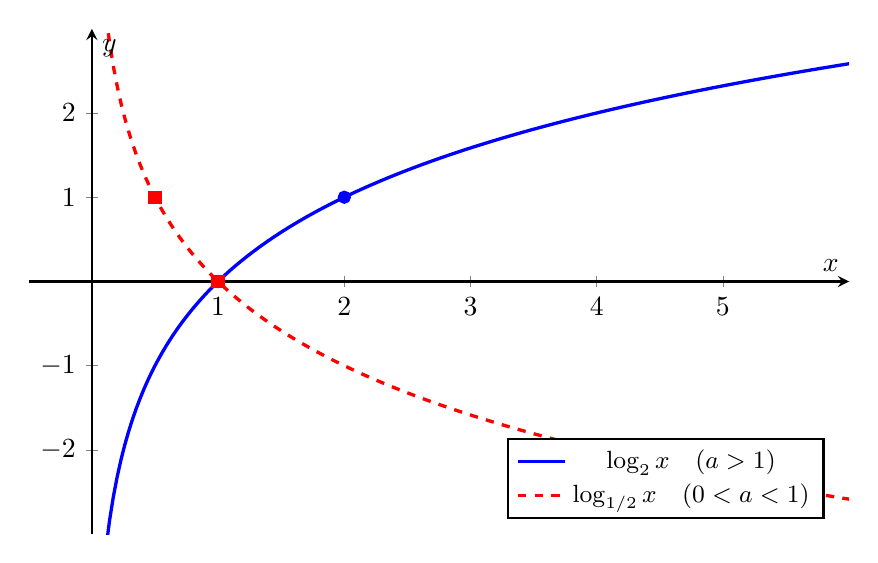
\begin{tikzpicture}
\begin{axis}[
  width=12cm, height=8cm,
  axis lines=center,
  xlabel={$x$}, ylabel={$y$},
  xmin=-0.5, xmax=6,
  ymin=-3, ymax=3,
  xtick={1,2,3,4,5},
  ytick={-2,-1,0,1,2},
  legend pos=south east,
  legend style={font=\small},
  samples=200,
  domain=0.05:6,
  thick
]
  % a > 1: log base 2
  \addplot[blue, very thick] {ln(x)/ln(2)};
  \addlegendentry{$\log_2 x \quad (a>1)$}

  % 0 < a < 1: log base 1/2
  \addplot[red, very thick, dashed] {ln(x)/ln(0.5)};
  \addlegendentry{$\log_{1/2} x \quad (0<a<1)$}

  % y = 0 reference
  \addplot[black, thin, dotted] coordinates {(0.05,0)(6,0)};

  % Key points
  \addplot[blue, only marks, mark=*, mark size=2pt]
    coordinates {(1,0) (2,1)};
  \addplot[red, only marks, mark=square*, mark size=2pt]
    coordinates {(1,0) (0.5,1)};
\end{axis}
\end{tikzpicture}
\end{center}

\subsubsection*{Grafiko transformacijos}

Remiantis bendrosiomis funkcijų transformacijos taisyklėmis, logaritminės funkcijos grafiką galima perkelti, išplėsti ar atspindėti [web:3][web:5]:

\begin{tcolorbox}[title={Transformacijų lentelė}]
\begin{tabular}{ll}
\textbf{Funkcija} & \textbf{Transformacija} \\[4pt]
$y = \log_a x + k$ & Poslinkis \textbf{vertikaliai}: $k$ vienetų aukštyn ($k>0$) arba žemyn ($k<0$) \\[4pt]
$y = \log_a(x - h)$ & Poslinkis \textbf{horizontaliai}: $h$ vienetų dešinėn ($h>0$) arba kairėn ($h<0$) \\
& Nauja vertikalioji asimptotė: $x = h$ \\[4pt]
$y = -\log_a x$ & \textbf{Atspindys} $x$ ašies atžvilgiu \\[4pt]
$y = \log_a(-x)$ & \textbf{Atspindys} $y$ ašies atžvilgiu; apibrėžimo sritis $(-\infty; 0)$ \\[4pt]
$y = k \cdot \log_a x$ & \textbf{Vertikalus ištempimas} ($|k|>1$) arba suspaudimas ($0<|k|<1$) \\[4pt]
$y = \log_a(kx)$ & \textbf{Horizontalus suspaudimas} (jei $k>1$); naudojant sandaugos taisyklę: \\
& $\log_a(kx) = \log_a k + \log_a x$ – tai poslinkis vertikaliai \\
\end{tabular}
\end{tcolorbox}

\begin{example}
Nubrėžkite funkcijos $y = \log_2(x - 3) + 1$ grafiko eskizą ir nurodykite jo savybes.

\textbf{Sprendimas:}
\begin{itemize}
  \item Pradedame nuo $y = \log_2 x$.
  \item Poslinkis 3 vienetais \textbf{dešinėn}: $y = \log_2(x-3)$.
  \item Poslinkis 1 vienetu \textbf{aukštyn}: $y = \log_2(x-3) + 1$.
  \item Nauja vertikalioji asimptotė: $x = 3$.
  \item Apibrėžimo sritis: $(3; +\infty)$.
  \item Grafikas kerta $x$ ašį, kai $\log_2(x-3)+1 = 0$, t.y. $x - 3 = 2^{-1}$, taigi $x = 3{,}5$.
  \item Reikšmių sritis: $\mathbb{R}$.
\end{itemize}
\end{example}

\begin{exercise}
Nustatykite, kuriam intervalui priklauso $x$, jei $y = \log_{0{,}5}(2x - 4) \geq 0$.

\textit{Patarimas:} Kadangi bazė $a = 0{,}5 < 1$, logaritmų funkcija \textbf{mažėja}, todėl nelygybės ženklas keičiasi, kai pereinate nuo logaritmų prie laipsnių.

\textbf{Sprendimas:}
Sąlyga $y \geq 0$ reiškia:
\[
  \log_{0{,}5}(2x-4) \geq 0 \iff 2x-4 \leq (0{,}5)^0 = 1 \quad (\text{ženklas keičiasi!})
\]
Be to, reikia $2x - 4 > 0$, t.y. $x > 2$. Taigi:
\[
  2x - 4 \leq 1 \implies x \leq 2{,}5.
\]
Atsakymas: $x \in (2;\ 2{,}5]$.
\end{exercise}


\section{Eksponentinės lygtys ir nelygybės}

Eksponentinės lygtys ir nelygybės yra tokios, kuriose nežinomasis $x$ yra laipsnio rodiklyje.
Sprendžiant jas remiamasi eksponentinės funkcijos savybėmis ir logaritmais.

% -------------------------------------------------------
\subsection{Eksponentinės lygtys}
% -------------------------------------------------------

\begin{definition}
\textbf{Eksponentinė lygtis} – lygtis, kurioje nežinomasis yra laipsnio rodiklyje.
Bendroji forma:
\[
    a^{f(x)} = a^{g(x)}, \quad a > 0,\ a \neq 1.
\]
\end{definition}

\subsubsection*{Pagrindinė sprendimo taisyklė}

Jei abiejų lygties pusių pagrindai vienodi ir $a > 0$, $a \neq 1$, tai:
\[
    a^{f(x)} = a^{g(x)} \iff f(x) = g(x).
\]

\begin{example}
Išspręskite lygtį $2^{3x-1} = 2^{x+5}$.

\textbf{Sprendimas.} Pagrindai vienodi ($a = 2$), todėl:
\[
    3x - 1 = x + 5 \implies 2x = 6 \implies x = 3.
\]
\textbf{Atsakymas:} $x = 3$.
\end{example}

\subsubsection*{Pagrindų sulyginimo metodas}

Kai pagrindai skirtingi, bet juos galima išreikšti vienodu pagrindu, abu pusę
perrašome naudodami tą patį pagrindą.

\begin{example}
Išspręskite lygtį $4^{x} = 8^{x-1}$.

\textbf{Sprendimas.} Pastebime, kad $4 = 2^2$ ir $8 = 2^3$:
\[
    (2^2)^{x} = (2^3)^{x-1}
    \implies 2^{2x} = 2^{3(x-1)}
    \implies 2x = 3x - 3
    \implies x = 3.
\]
\textbf{Atsakymas:} $x = 3$.
\end{example}

\begin{example}
Išspręskite lygtį $9^{x} - 4 \cdot 3^{x} + 3 = 0$.

\textbf{Sprendimas.} Pastebime, kad $9^x = (3^2)^x = (3^x)^2$.
Įveskime keitinį $t = 3^x$, $t > 0$:
\[
    t^2 - 4t + 3 = 0.
\]
Diskriminantas: $D = 16 - 12 = 4$, todėl:
\[
    t_1 = \frac{4 + 2}{2} = 3, \quad t_2 = \frac{4 - 2}{2} = 1.
\]
Grįžtame prie originalo:
\[
    3^x = 3 \implies x = 1; \qquad 3^x = 1 = 3^0 \implies x = 0.
\]
\textbf{Atsakymas:} $x_1 = 0$, $x_2 = 1$.
\end{example}

\subsubsection*{Sprendimas logaritmavimu}

Jei pagrindų sulyginimas nėra įmanomas, naudojamas logaritmavimas. Logaritmuojame
abi lygties puses:
\[
    a^x = b \implies x \ln a = \ln b \implies x = \frac{\ln b}{\ln a} = \log_a b.
\]

\begin{example}
Išspręskite lygtį $3^x = 7$.

\textbf{Sprendimas.}
\[
    x = \log_3 7 = \frac{\ln 7}{\ln 3} \approx \frac{1{,}946}{1{,}099} \approx 1{,}771.
\]
\textbf{Atsakymas:} $x = \log_3 7$.
\end{example}

\subsubsection*{Eksponentinės lygčių sistemos}

VBE egzamine gali pasitaikyti eksponentinių lygčių sistemos, kurias paprasčiausias sprendimas
yra pagrindų sulyginimas arba padalijimas.

\begin{example}
Išspręskite sistemą:
\[
    \begin{cases}
        2^x \cdot 2^y = 64, \\
        2^x \div 2^y = 4.
    \end{cases}
\]

\textbf{Sprendimas.} Pirmąją lygtį supaprastiname:
\[
    2^{x+y} = 2^6 \implies x + y = 6.
\]
Antrąją lygtį supaprastiname:
\[
    2^{x-y} = 2^2 \implies x - y = 2.
\]
Sudedame: $2x = 8 \implies x = 4$. Tada $y = 2$.\\
\textbf{Atsakymas:} $x = 4$, $y = 2$.
\end{example}

\begin{tcolorbox}[title={Eksponentinių lygčių sprendimo algoritmas}]
\begin{enumerate}
    \item Patikrinkite, ar galima sulyginiti pagrindus (pvz., $4 = 2^2$, $8 = 2^3$, $27 = 3^3$).
    \item Jei ne, naudokite keitinį $t = a^x$ (jei lygtis kvadratinė pagal $a^x$).
    \item Jei nei vienas metodas netinka – logaritmuokite abi puses.
    \item Patikrinkite sprendinius (ypač po keitinio: $t > 0$).
\end{enumerate}
\end{tcolorbox}

\subsubsection*{Dažniausiai VBE naudojami pagrindai}

\[
\begin{array}{c|c}
    \textbf{Skaičius} & \textbf{Išraiška} \\
    \hline
    4 & 2^2 \\
    8 & 2^3 \\
    16 & 2^4 \\
    32 & 2^5 \\
    9 & 3^2 \\
    27 & 3^3 \\
    25 & 5^2 \\
    0{,}5 & 2^{-1} \\
    0{,}25 & 2^{-2} \\
    \tfrac{1}{3} & 3^{-1} \\
\end{array}
\]

% -------------------------------------------------------
\subsection{Eksponentinės nelygybės}
% -------------------------------------------------------

\begin{definition}
\textbf{Eksponentinė nelygybė} – nelygybė, kurioje nežinomasis yra laipsnio rodiklyje.
Bendroji forma: $a^{f(x)} > a^{g(x)}$ (arba su $<$, $\geq$, $\leq$).
\end{definition}

\subsubsection*{Pagrindinė sprendimo taisyklė}

Eksponentinės nelygybės sprendimas priklauso nuo pagrindo $a$ reikšmės:

\begin{tcolorbox}[title={Eksponentinės nelygybės savybės}]
\[
    \text{Jei } a > 1: \quad a^{f(x)} > a^{g(x)} \iff f(x) > g(x).
\]
\[
    \text{Jei } 0 < a < 1: \quad a^{f(x)} > a^{g(x)} \iff f(x) < g(x).
\]
Kai $0 < a < 1$, nelygybės kryptis \textbf{apsiverčia}!
\end{tcolorbox}

\textbf{Intuicija:} Kai $a > 1$, funkcija $y = a^x$ yra didėjanti, todėl didesnis
rodiklis duoda didesnę reikšmę. Kai $0 < a < 1$, funkcija $y = a^x$ yra mažėjanti,
todėl didesnis rodiklis duoda \emph{mažesnę} reikšmę.

\begin{example}
Išspręskite nelygybę $3^{2x-1} > 3^{x+3}$.

\textbf{Sprendimas.} Pagrindas $a = 3 > 1$, todėl kryptis nesikeičia:
\[
    2x - 1 > x + 3 \implies x > 4.
\]
\textbf{Atsakymas:} $x \in (4; +\infty)$.
\end{example}

\begin{example}
Išspręskite nelygybę $\left(\dfrac{1}{2}\right)^{x+2} \leq \left(\dfrac{1}{2}\right)^{3x-4}$.

\textbf{Sprendimas.} Pagrindas $a = \tfrac{1}{2} \in (0;\, 1)$, todėl nelygybės kryptis apsiverčia:
\[
    x + 2 \geq 3x - 4 \implies -2x \geq -6 \implies x \leq 3.
\]
\textbf{Atsakymas:} $x \in (-\infty;\, 3]$.
\end{example}

\begin{example}
Išspręskite nelygybę $4^{x} \leq 8$.

\textbf{Sprendimas.} Išreiškiame vienodu pagrindu ($2$):
\[
    (2^2)^x \leq 2^3 \implies 2^{2x} \leq 2^3.
\]
Kadangi $a = 2 > 1$, kryptis nesikeičia:
\[
    2x \leq 3 \implies x \leq \frac{3}{2}.
\]
\textbf{Atsakymas:} $x \in \left(-\infty;\, \dfrac{3}{2}\right]$.
\end{example}

\begin{example}
Išspręskite nelygybę $9^x - 10 \cdot 3^x + 9 \leq 0$.

\textbf{Sprendimas.} Taikome keitinį $t = 3^x > 0$. Tada $9^x = t^2$:
\[
    t^2 - 10t + 9 \leq 0.
\]
Randame šaknis: $t^2 - 10t + 9 = 0 \implies (t-1)(t-9) = 0$, todėl $t_1 = 1$, $t_2 = 9$.\\
Kadangi koeficientas prie $t^2$ teigiamas, kvadratinis trinaris $\leq 0$ intervale $[1;\, 9]$.\\
Todėl:
\[
    1 \leq 3^x \leq 9 \implies 3^0 \leq 3^x \leq 3^2 \implies 0 \leq x \leq 2.
\]
\textbf{Atsakymas:} $x \in [0;\, 2]$.
\end{example}

\begin{example}
Išspręskite nelygybę $2^{x+3} - 2^x > 3$.

\textbf{Sprendimas.} Išskiriame $2^x$:
\[
    2^x \cdot 2^3 - 2^x > 3 \implies 2^x(8 - 1) > 3 \implies 7 \cdot 2^x > 3
    \implies 2^x > \frac{3}{7}.
\]
Logaritmuojame (pagrindas $2 > 1$):
\[
    x > \log_2\frac{3}{7} = \log_2 3 - \log_2 7.
\]
\textbf{Atsakymas:} $x \in \left(\log_2 3 - \log_2 7;\, +\infty\right)$.
\end{example}

\subsubsection*{Sprendimo algoritmo santrauka}

\begin{tcolorbox}[title={Eksponentinių nelygybių sprendimo algoritmas}]
\begin{enumerate}
    \item Sulyginame pagrindus (jei įmanoma).
    \item Jei lygtis kvadratinė pagal $a^x$ – taikome keitinį $t = a^x > 0$.
    \item Rašome rodiklių nelygybę, \textbf{atsižvelgdami į pagrindo dydį}:
    \begin{itemize}
        \item $a > 1$: kryptis \textbf{nesikeičia};
        \item $0 < a < 1$: kryptis \textbf{apsiverčia}.
    \end{itemize}
    \item Sprendžiame gautą algebrinę nelygybę.
    \item Užrašome atsakymą intervalo forma.
\end{enumerate}
\end{tcolorbox}

\subsubsection*{Tipiški VBE klausimai}

\begin{exercise}
Išspręskite nelygybę $5^{2x+1} \geq 125$.
\end{exercise}
\begin{proof}[Sprendimas]
$5^{2x+1} \geq 5^3 \implies 2x + 1 \geq 3 \implies x \geq 1$.
Atsakymas: $x \in [1;\, +\infty)$.
\end{proof}

\begin{exercise}
Išspręskite nelygybę $\left(\dfrac{1}{3}\right)^{2x-1} < \dfrac{1}{27}$.
\end{exercise}
\begin{proof}[Sprendimas]
$\dfrac{1}{27} = \left(\dfrac{1}{3}\right)^3$, todėl:
$\left(\dfrac{1}{3}\right)^{2x-1} < \left(\dfrac{1}{3}\right)^3$.
Kadangi $0 < a = \tfrac{1}{3} < 1$, kryptis apsiverčia:
$2x - 1 > 3 \implies x > 2$.
Atsakymas: $x \in (2;\, +\infty)$.
\end{proof}

\begin{exercise}
Eksponentinė lygtis su absoliučia verte: išspręskite $2^{|x|} = 16$.
\end{exercise}
\begin{proof}[Sprendimas]
$2^{|x|} = 2^4 \implies |x| = 4 \implies x = \pm 4$.
Atsakymas: $x \in \{-4;\, 4\}$.
\end{proof}


\section{Logaritminės lygtys ir nelygybės}

\subsection{Logaritminės lygtys}

\begin{definition}
\textbf{Logaritminė lygtis} — tai lygtis, kurioje nežinomasis yra logaritmo argumente, pagrinde arba abiejose vietose. Bendroji forma:
\[
\log_a f(x) = \log_a g(x) \quad \text{arba} \quad \log_a f(x) = b,
\]
kur \(a > 0\), \(a \neq 1\).
\end{definition}

\subsubsection{Egzistavimo sąlygos (ODR)}

Prieš sprendžiant bet kurią logaritminę lygtį, \textbf{būtina} nustatyti leistinų reikšmių sritį (ODR). Logaritmas \(\log_a f(x)\) egzistuoja tik tada, kai:
\[
f(x) > 0 \quad \text{ir} \quad a > 0, \quad a \neq 1.
\]

\begin{tcolorbox}[colback=yellow!10, colframe=orange!60, title=\textbf{Svarbu! ODR tikrinimas}]
Visuomet patikrinkite gautus sprendinius — logaritmo argumentas \textbf{visada} turi būti teigiamas skaičius. Sprendiniai, netenkinantys ODR, atmetami.
\end{tcolorbox}

\subsubsection{I metodas: Logaritmo apibrėžimo taikymas}

Jei lygtis yra pavidalo \(\log_a f(x) = b\), ją galima pertvarkyti į rodiklinę lygtį:
\[
\log_a f(x) = b \iff f(x) = a^b.
\]

\begin{example}
Išspręskite lygtį \(\log_3(x - 2) = 3\).

\textbf{Sprendimas:}
\begin{align*}
&\text{ODR: } x - 2 > 0 \implies x > 2.\\
&\log_3(x-2) = 3 \iff x - 2 = 3^3 = 27 \implies x = 29.
\end{align*}
Patikriname: \(x = 29 > 2\) — tinka.

\textbf{Atsakymas:} \(x = 29\).
\end{example}

\subsubsection{II metodas: Antilogaritmavimas (vienodų pagrindų taisyklė)}

Jei abu lygties nariai yra logaritmai tuo pačiu pagrindu, taikome savybę:
\[
\log_a f(x) = \log_a g(x) \iff f(x) = g(x),
\]
tačiau \textbf{būtina} papildomai patikrinti ODR sąlygas.

\begin{example}
Išspręskite lygtį \(\log_5(2x + 1) = \log_5(x + 4)\).

\textbf{Sprendimas:}
\begin{align*}
&\text{ODR: } 2x + 1 > 0 \text{ ir } x + 4 > 0 \implies x > -\tfrac{1}{2}.\\
&2x + 1 = x + 4 \implies x = 3.
\end{align*}
Patikriname: \(x = 3 > -\tfrac{1}{2}\) — tinka.

\textbf{Atsakymas:} \(x = 3\).
\end{example}

\subsubsection{III metodas: Logaritmų savybių taikymas}

Sudėtingesnėse lygtyse pirmiausia supaprastiname išraišką naudodami logaritmų savybes:
\begin{align*}
\log_a(mn) &= \log_a m + \log_a n,\\
\log_a\!\left(\frac{m}{n}\right) &= \log_a m - \log_a n,\\
\log_a m^k &= k \cdot \log_a m.
\end{align*}

\begin{example}
Išspręskite lygtį \(\log_2 x + \log_2(x - 2) = 3\).

\textbf{Sprendimas:}
\begin{align*}
&\text{ODR: } x > 0 \text{ ir } x - 2 > 0 \implies x > 2.\\
&\log_2\bigl(x(x-2)\bigr) = 3 \iff x(x-2) = 2^3 = 8.\\
&x^2 - 2x - 8 = 0.\\
&(x-4)(x+2) = 0 \implies x_1 = 4,\quad x_2 = -2.
\end{align*}
Patikriname: \(x_2 = -2\) neatitinka ODR (\(x > 2\)), todėl atmetamas.

\textbf{Atsakymas:} \(x = 4\).
\end{example}

\begin{example}
Išspręskite lygtį \(\log_3(x+1) - \log_3(x-2) = 2\).

\textbf{Sprendimas:}
\begin{align*}
&\text{ODR: } x + 1 > 0 \text{ ir } x - 2 > 0 \implies x > 2.\\
&\log_3\!\left(\frac{x+1}{x-2}\right) = 2 \iff \frac{x+1}{x-2} = 9.\\
&x + 1 = 9(x-2) = 9x - 18 \implies -8x = -19 \implies x = \frac{19}{8} = 2{,}375.
\end{align*}
Patikriname: \(x = 2{,}375 > 2\) — tinka.

\textbf{Atsakymas:} \(x = \dfrac{19}{8}\).
\end{example}

\subsubsection{IV metodas: Keitinys}

Kai logaritminė lygtis turi sudėtingą struktūrą (pvz., lygtis panaši į kvadratinę pagal logaritmą), taikomas \textbf{keitinys} \(t = \log_a f(x)\).

\begin{example}
Išspręskite lygtį \(\left(\log_2 x\right)^2 - 3\log_2 x + 2 = 0\).

\textbf{Sprendimas.} Pažymime \(t = \log_2 x\). Tada:
\[
t^2 - 3t + 2 = 0 \implies (t-1)(t-2) = 0.
\]
\[
t_1 = 1 \implies \log_2 x = 1 \implies x_1 = 2.
\]
\[
t_2 = 2 \implies \log_2 x = 2 \implies x_2 = 4.
\]
Abiem atvejais \(x > 0\) — tinka.

\textbf{Atsakymas:} \(x_1 = 2\), \(x_2 = 4\).
\end{example}

\begin{tcolorbox}[colback=blue!5, colframe=blue!40, title=\textbf{Logaritminių lygčių sprendimo žingsniai}]
\begin{enumerate}
    \item Nustatyti ODR (leistinų reikšmių sritį).
    \item Pasirinkti tinkamą sprendimo metodą:
    \begin{itemize}
        \item Tiesioginis: \(\log_a f(x) = b \iff f(x) = a^b\),
        \item Antilogaritmavimas: \(\log_a f(x) = \log_a g(x) \iff f(x) = g(x)\),
        \item Logaritmų savybės (sandaugos, dalybos, laipsnio),
        \item Keitinys.
    \end{itemize}
    \item Gauti sprendiniai patikrinami pagal ODR sąlygas.
\end{enumerate}
\end{tcolorbox}

\begin{exercise}
Išspręskite lygtis:
\begin{enumerate}[label=\alph*)]
    \item \(\log_4(3x - 5) = 2\)
    \item \(\log_6 x + \log_6(x+1) = 1\)
    \item \(\log_5(x+3) - \log_5(x-1) = 1\)
    \item \((\log_3 x)^2 - 4\log_3 x + 3 = 0\)
    \item \(\log_2(x^2 - 4x + 4) = 2\)
\end{enumerate}
\end{exercise}

% -------------------------------------------------------
\subsection{Logaritminės nelygybės}
% -------------------------------------------------------

\begin{definition}
\textbf{Logaritminė nelygybė} — tai nelygybė, kurioje nežinomasis randasi logaritmo argumente. Bendroji forma:
\[
\log_a f(x) > \log_a g(x), \quad \log_a f(x) < b, \quad \text{ir pan.}
\]
\end{definition}

\subsubsection{Pagrindinis sprendimo principas: monotonija}

Logaritminės funkcijos \(y = \log_a x\) monotonija priklauso nuo pagrindo \(a\):

\begin{tcolorbox}[colback=green!5, colframe=green!40, title=\textbf{Nelygybės krypties taisyklė}]
\begin{itemize}
    \item Kai \(a > 1\): \(\log_a f(x) > \log_a g(x) \iff f(x) > g(x)\) \quad (\textbf{kryptis nesikeičia}).
    \item Kai \(0 < a < 1\): \(\log_a f(x) > \log_a g(x) \iff f(x) < g(x)\) \quad (\textbf{kryptis keičiasi}).
\end{itemize}
Abiem atvejais \textbf{būtina} sąlyga: \(f(x) > 0\) ir \(g(x) > 0\).
\end{tcolorbox}

\subsubsection{I tipas: Paprasta logaritminė nelygybė}

\begin{example}
Išspręskite nelygybę \(\log_3(2x - 4) > 2\).

\textbf{Sprendimas:}
\begin{align*}
&\text{ODR: } 2x - 4 > 0 \implies x > 2.\\
&\log_3(2x-4) > 2 = \log_3 9 \iff 2x - 4 > 9 \implies x > \frac{13}{2}.
\end{align*}
Atsižvelgus į ODR: \(x > \dfrac{13}{2}\).

\textbf{Atsakymas:} \(x \in \left(\dfrac{13}{2};\, +\infty\right)\).
\end{example}

\begin{example}
Išspręskite nelygybę \(\log_{1/2}(x + 1) > \log_{1/2}(3 - x)\).

\textbf{Sprendimas:}
\begin{align*}
&\text{ODR: } x + 1 > 0 \text{ ir } 3 - x > 0 \implies -1 < x < 3.\\
&\text{Kadangi pagrindas } \tfrac{1}{2} < 1, \text{ nelygybės kryptis keičiasi:}\\
&x + 1 < 3 - x \implies 2x < 2 \implies x < 1.
\end{align*}
Atsižvelgus į ODR: \(-1 < x < 1\).

\textbf{Atsakymas:} \(x \in (-1;\, 1)\).
\end{example}

\subsubsection{II tipas: Nelygybė su logaritmų savybėmis}

\begin{example}
Išspręskite nelygybę \(\log_2 x + \log_2(x - 3) < 2\).

\textbf{Sprendimas:}
\begin{align*}
&\text{ODR: } x > 0 \text{ ir } x - 3 > 0 \implies x > 3.\\
&\log_2\bigl(x(x-3)\bigr) < 2 = \log_2 4 \iff x(x-3) < 4.\\
&x^2 - 3x - 4 < 0 \implies (x-4)(x+1) < 0 \implies -1 < x < 4.
\end{align*}
Atsižvelgus į ODR (\(x > 3\)): \(3 < x < 4\).

\textbf{Atsakymas:} \(x \in (3;\, 4)\).
\end{example}

\subsubsection{III tipas: Kvadratinė nelygybė pagal logaritmą (keitinys)}

\begin{example}
Išspręskite nelygybę \((\log_2 x)^2 - \log_2 x - 2 < 0\).

\textbf{Sprendimas.} Pažymime \(t = \log_2 x\) (su ODR sąlyga \(x > 0\)):
\[
t^2 - t - 2 < 0 \implies (t-2)(t+1) < 0 \implies -1 < t < 2.
\]
Grįžtame prie nežinomojo \(x\):
\[
-1 < \log_2 x < 2 \iff 2^{-1} < x < 2^2 \implies \frac{1}{2} < x < 4.
\]

\textbf{Atsakymas:} \(x \in \left(\dfrac{1}{2};\, 4\right)\).
\end{example}

\subsubsection{Sprendimo schemos palyginimas}

\begin{center}
\begin{tabular}{|p{4.2cm}|p{4.8cm}|p{4.8cm}|}
\hline
\textbf{Nelygybės tipas} & \textbf{Pagrindas } \(a > 1\) & \textbf{Pagrindas } \(0 < a < 1\)\\
\hline
\(\log_a f(x) > b\) & \(f(x) > a^b\) & \(0 < f(x) < a^b\)\\
\hline
\(\log_a f(x) < b\) & \(0 < f(x) < a^b\) & \(f(x) > a^b\)\\
\hline
\(\log_a f(x) > \log_a g(x)\) & \(f(x) > g(x) > 0\) & \(0 < f(x) < g(x)\)\\
\hline
\(\log_a f(x) < \log_a g(x)\) & \(0 < f(x) < g(x)\) & \(f(x) > g(x) > 0\)\\
\hline
\end{tabular}
\end{center}

\begin{tcolorbox}[colback=blue!5, colframe=blue!40, title=\textbf{Logaritminių nelygybių sprendimo žingsniai}]
\begin{enumerate}
    \item Nustatyti ODR: visi logaritmų argumentai turi būti \textbf{teigiami}.
    \item Supaprastinti išraiškas naudojant logaritmų savybes.
    \item Pertvarkyti nelygybę atsižvelgiant į pagrindo vertę (\(a > 1\) arba \(0 < a < 1\)).
    \item Išspręsti gautą algebrinę nelygybę.
    \item \textbf{Susikirtimas} su ODR — galutinis atsakymas.
\end{enumerate}
\end{tcolorbox}

\begin{exercise}
Išspręskite nelygybes:
\begin{enumerate}[label=\alph*)]
    \item \(\log_5(3x - 1) < 2\)
    \item \(\log_{1/3}(x + 2) \geq \log_{1/3}(2x - 1)\)
    \item \(\log_4 x + \log_4(x + 6) \leq 2\)
    \item \((\log_3 x)^2 - 2\log_3 x - 3 \geq 0\)
    \item \(\log_2(x^2 - 5x + 6) > 1\)
\end{enumerate}
\end{exercise}

